\documentclass{article}
\usepackage[utf8]{inputenc}
\usepackage[a4paper, total={7.8in, 11.5in}]{geometry}
\usepackage{graphicx}
\graphicspath{ {./images/} }

\title{Privacy Focussed Self Improving Disaster Detection Using A Distributed Network}
\author{Josh Pattman - Supervised by Mohammad Soorati}

\begin{document}
\maketitle

\section{Problem}
Disasters, such as house fires and car crashes, are an unfortunate yet frequent part of our lives in the modern world. Today, we still rely heavily upon passers by to call emergency services, and dispatch help to the situation. However, this is not only slow, but it can also be difficult to understand a panicked citizen who could give the emergency services incorrect information in their fluster. In a disaster situation, every second counts, so any improvement to this system could save lives.

\section{Proposal}
\emph{From this point on an internet connected device with a camera and known position and orientation will be referred to as an agent.}
\subsection{Goals}
Today, there are a multitude of devices that are capable of acting as agents. From smartphones to doorbell cameras to consumer drones, most areas of a modern city are under constant surveillance. However, due to privacy protection, it is inviable to stream this video to any location other than the device. The goals of this project are to: Report disasters as fast as possible, protect the privacy of any user who's device is being used as an agent, improve the systems response speed over time, and finally have exceptional fault tolerance.


\subsection{Scope}
This project will include development of the machine learning and fusing algorithm. It will provide access to these through simple command line tools and python notebooks. There will be no user interface created that could be used in real life, as this is out of scope of the project. Also, for a large portion of the experimentation phase, a simulation will be used to generate camera feeds around an area. At later stages, real life images may be used, however these will be far harder to come by, so may not be possible. The project will also entail running the algorithms on one or multiple computers on the same network, however the code will not be implemented onto actual devices such as doorbells or phones.

\subsection{Proposed solution}
\begin{center}
	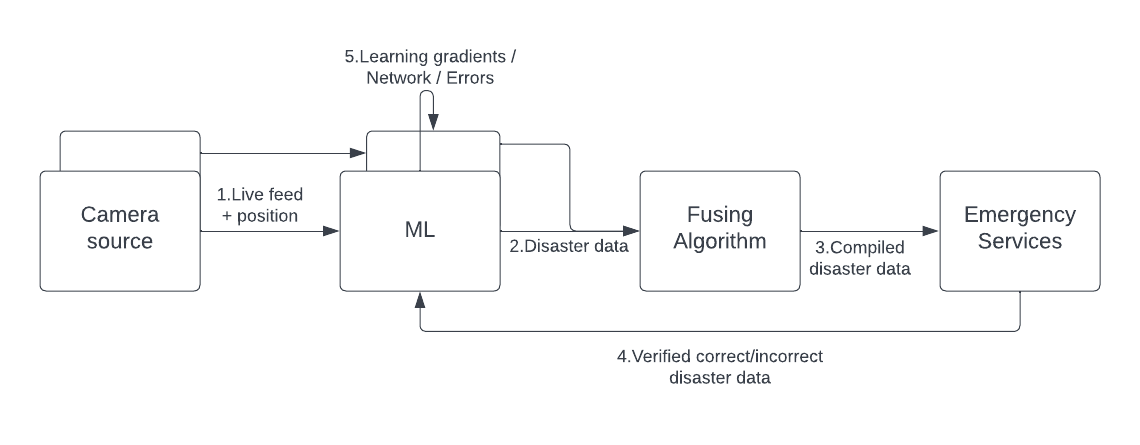
\includegraphics[scale=0.75]{proj}
\end{center}

\subsection{Phases}
\begin{enumerate}
	\item \textbf{Phase 1:} A photo-realistic simulation will be created. It will stream in-simulation camera feeds to the various agents.
	\item \textbf{Phase 2:} A single agent will be trained on video from the simulation to predict locations of accidents in 3D space.
	\item \textbf{Phase 3:} Various video feeds from the simulation will be converted to 3D disaster coordinates, using the multiple copies of the trained agent from \emph{phase 2}. This data will be fed into the fusing algorithm to create a 3D map of disasters.
	\item \textbf{Phase 3:} An automatic feedback system will be created where the network of agents predict the position of disasters, and the data is then sent back to the simulation. The simulation then confirms or denies the existence of each disaster, which is forwarded to each agent on the network. Each agent then learns from this.
	\item \textbf{Phase 4:} Phase 3 will be repeated with real world data, however the agents from Phase 3 will be used as a starting point.
\end{enumerate}

\end{document}
